\begin{frame}[t]{Die Messbruecke - Abgleich der Messbruecke} 
    
    \begin{spacing}{0.9} \begin{tiny}
      \begin{table}[h!]
      \begin{tabular}{p{10cm} }
        \hline
        \textbf{Definition des Messbereichs} \\
        \hline \\
        \begin{minipage}{\textwidth}
           \begin{itemize}
               \item Unsere Temperaturmessbruecke mit einem 8Bit AD-Wandler digitalisiert werden
               \item 254 Schritte
               \item quadratische Approximation bis $100$C genau
               \item wir wählen eine Schrittweite von $0,5$C
           \end{itemize}
           Somit ergibt sich ein Temperaturbereich von $-27$C bist $100,5$C und die folgende Anforderung an unser Schaltung.\newline\newline
           \textbf{Die Messbrücke soll bei $-27$C abgeglichen sein.}
           \begin{itemize}
               \item Der KTY81-210 hat laut Datenblatt einen bei -27C Widerstand von $1282\Omega$
               \item $R_4$ muss daher $1282\Omega$ betragen
               \item In der Realität würde man einen $1k\Omega$ und einen auf $282\Omega$ getrimmten $500\Omega$-Trimmer verwenden
               \item In unserer Simulation reicht ein einfacher Widerstand mit $1282\Omega$ aus.
           \end{itemize}
           \begin{figure}
               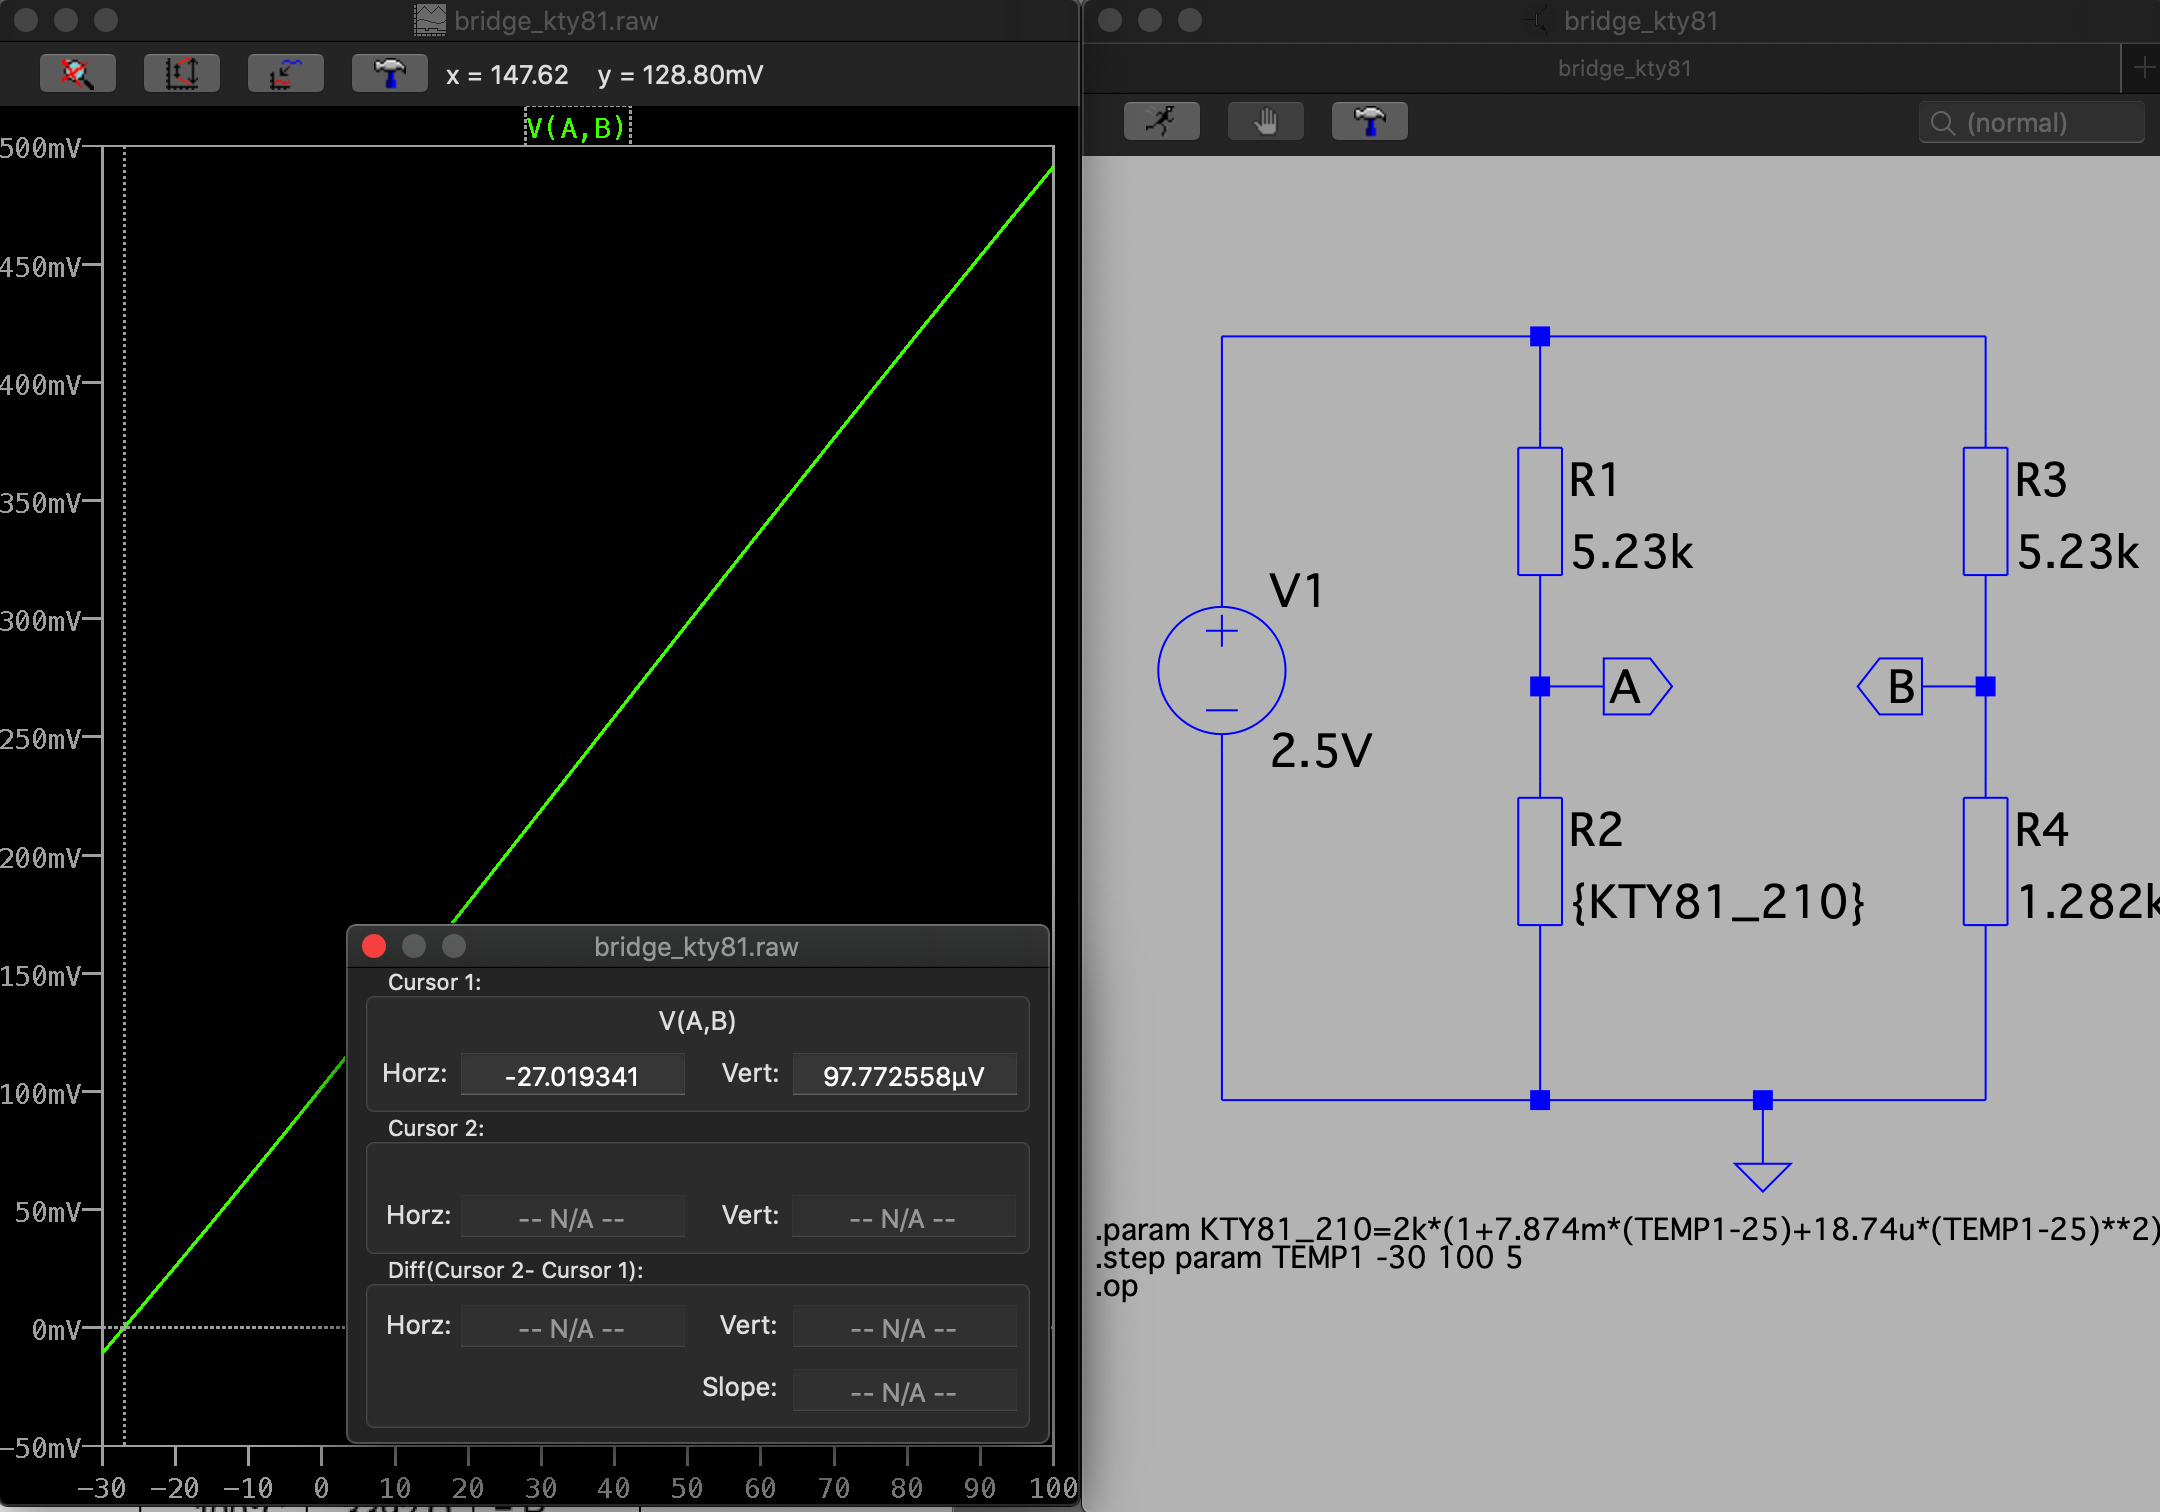
\includegraphics[width=0.5\linewidth]{pictures/kty81_getrimmet.png}
           \end{figure}
        \end{minipage}
       \\        
    \end{tabular}

    \end{table}
     
    \end{tiny} \end{spacing}

\end{frame}

\begin{frame}[t]{Die Messbruecke - Anpassung an AD-Wandler} 
    
    \begin{spacing}{0.9} \begin{tiny}
      \begin{table}[h!]
      \begin{tabular}{p{10cm} }
        \hline
        \textbf{Ausnutzung des Quantisierungsbereiches des AD-Wandlers} \\
        \hline \\
        \begin{minipage}{\textwidth}
           \begin{itemize}
               \item Der AD-Wandler hat eine Referenzspannung von 2,5V
               \item In der vorherigen Folie sehen wir, dass die Spannung der Messbrücke von 0 bis etwa 500mV reicht
               \item Zur Ausnutzung des kompletten Quantisierungsbereiches des AD-Wandlers muss die Brückenspannung auf 2,5V bei 100,5C verstärkt werden
           \end{itemize}
           \textbf{Hierzu werden wir einen Differenzverstärker verwenden}
        \end{minipage} 
        \\  \\
        \hline
        \textbf{Exkurs Differenzverstärker} \\
        \hline \\   
        \begin{tabular}{p{5cm} p{5cm}}
            \begin{minipage}{0.5\textwidth}
                \begin{figure}[h!]                
                    \scalebox{0.6}{
                    \centering
                    \begin{circuitikz}
                        \draw
                        (0, 0) node[op amp] (opamp) {}
                        (opamp.-) to[R,l=$R_1$] (-3, 0.5) to[short,-*,l=$V_a$] ++ (-1,0) 
                        (opamp.+) to[R,l=$R_2$] (-3, -0.5) to[short,-*,l=$V_b$] ++ (-0.5,0)
                        (opamp.-) to[short] ++(0,1.5) coordinate (leftR)
                        to[R,l=$R_k$] (leftR -| opamp.out)            
                        to[short] (opamp.out) to[short,-*,l=$U_{ADC}$] ++ (0.5,0)
                        (opamp.+) to[R,l=$R_q$] (-1.2,-2) node[ground]{};
                      \end{circuitikz}
                    }
                    \end{figure}
            \end{minipage}
            &
            \begin{minipage}{0.4\textwidth}
                Wenn gilt:\newline
                \begin{equation}
                    V_{D} = \frac{R_k}{R_1} = \frac{R_q}{R_2} 
                \end{equation}
                Dann ist der Differenzverstärker symmetrisch und kann mit der folgenden Formel dimensioniert werden.\newline
                \begin{equation}
                    U_{ADC}=V_{D}(V_b-V_a)
                \end{equation}
                Um die folgenden Berechnungen zu vereinfachen verwenden wir einen symmetrischen Differenzverstärker.
            \end{minipage}
        \end{tabular}

    \end{tabular}

    \end{table}
     
    \end{tiny} \end{spacing}

\end{frame}

\begin{frame}[t]{Die Messbruecke - Anpassung an AD-Wandler} 
    
    \begin{spacing}{0.9} \begin{tiny}
      \begin{table}[h!]
      \begin{tabular}{p{10cm} }
        \hline
        \textbf{Dimensionierung Differenzverstärker} \\
        \hline \\
        \begin{minipage}{\textwidth}
           \begin{itemize}
               \item Aus unserer Simulation (Folie 45) wissen wir, dass die Spannung $V_{AB}$ bei 100C 493mV entspricht
               \item Die Referenzspannung des AD-Wandler ist 2,5V 
               \item Das ergibt einen Verstärkungsfaktor $V_D=\frac{2,5}{0,493}=\thicksim 5,1$
               \item Wir wählen daher $R_k=R_q=480k\Omega$ sowie $R_1=R_2=91k\Omega$ 
           \end{itemize}
        \end{minipage} 
        \\\\
        \hline
        \textbf{Aufbau des Differenzverstärkers und Integration} \\
        \hline \\
        \begin{minipage}{\textwidth}
            Zur einfacheren Versorgung (eine 5V Versorgung für alles anstatt einer zusätzlichen +/-12V Versorgung)
            verwenden wir den UniversalOpamp2 im unsymmetrischen Modus von 5V bis 0V. Dies reicht aus, da unser Messbereich
            von 0-2,5V reicht.
            \begin{figure}
                \centering
                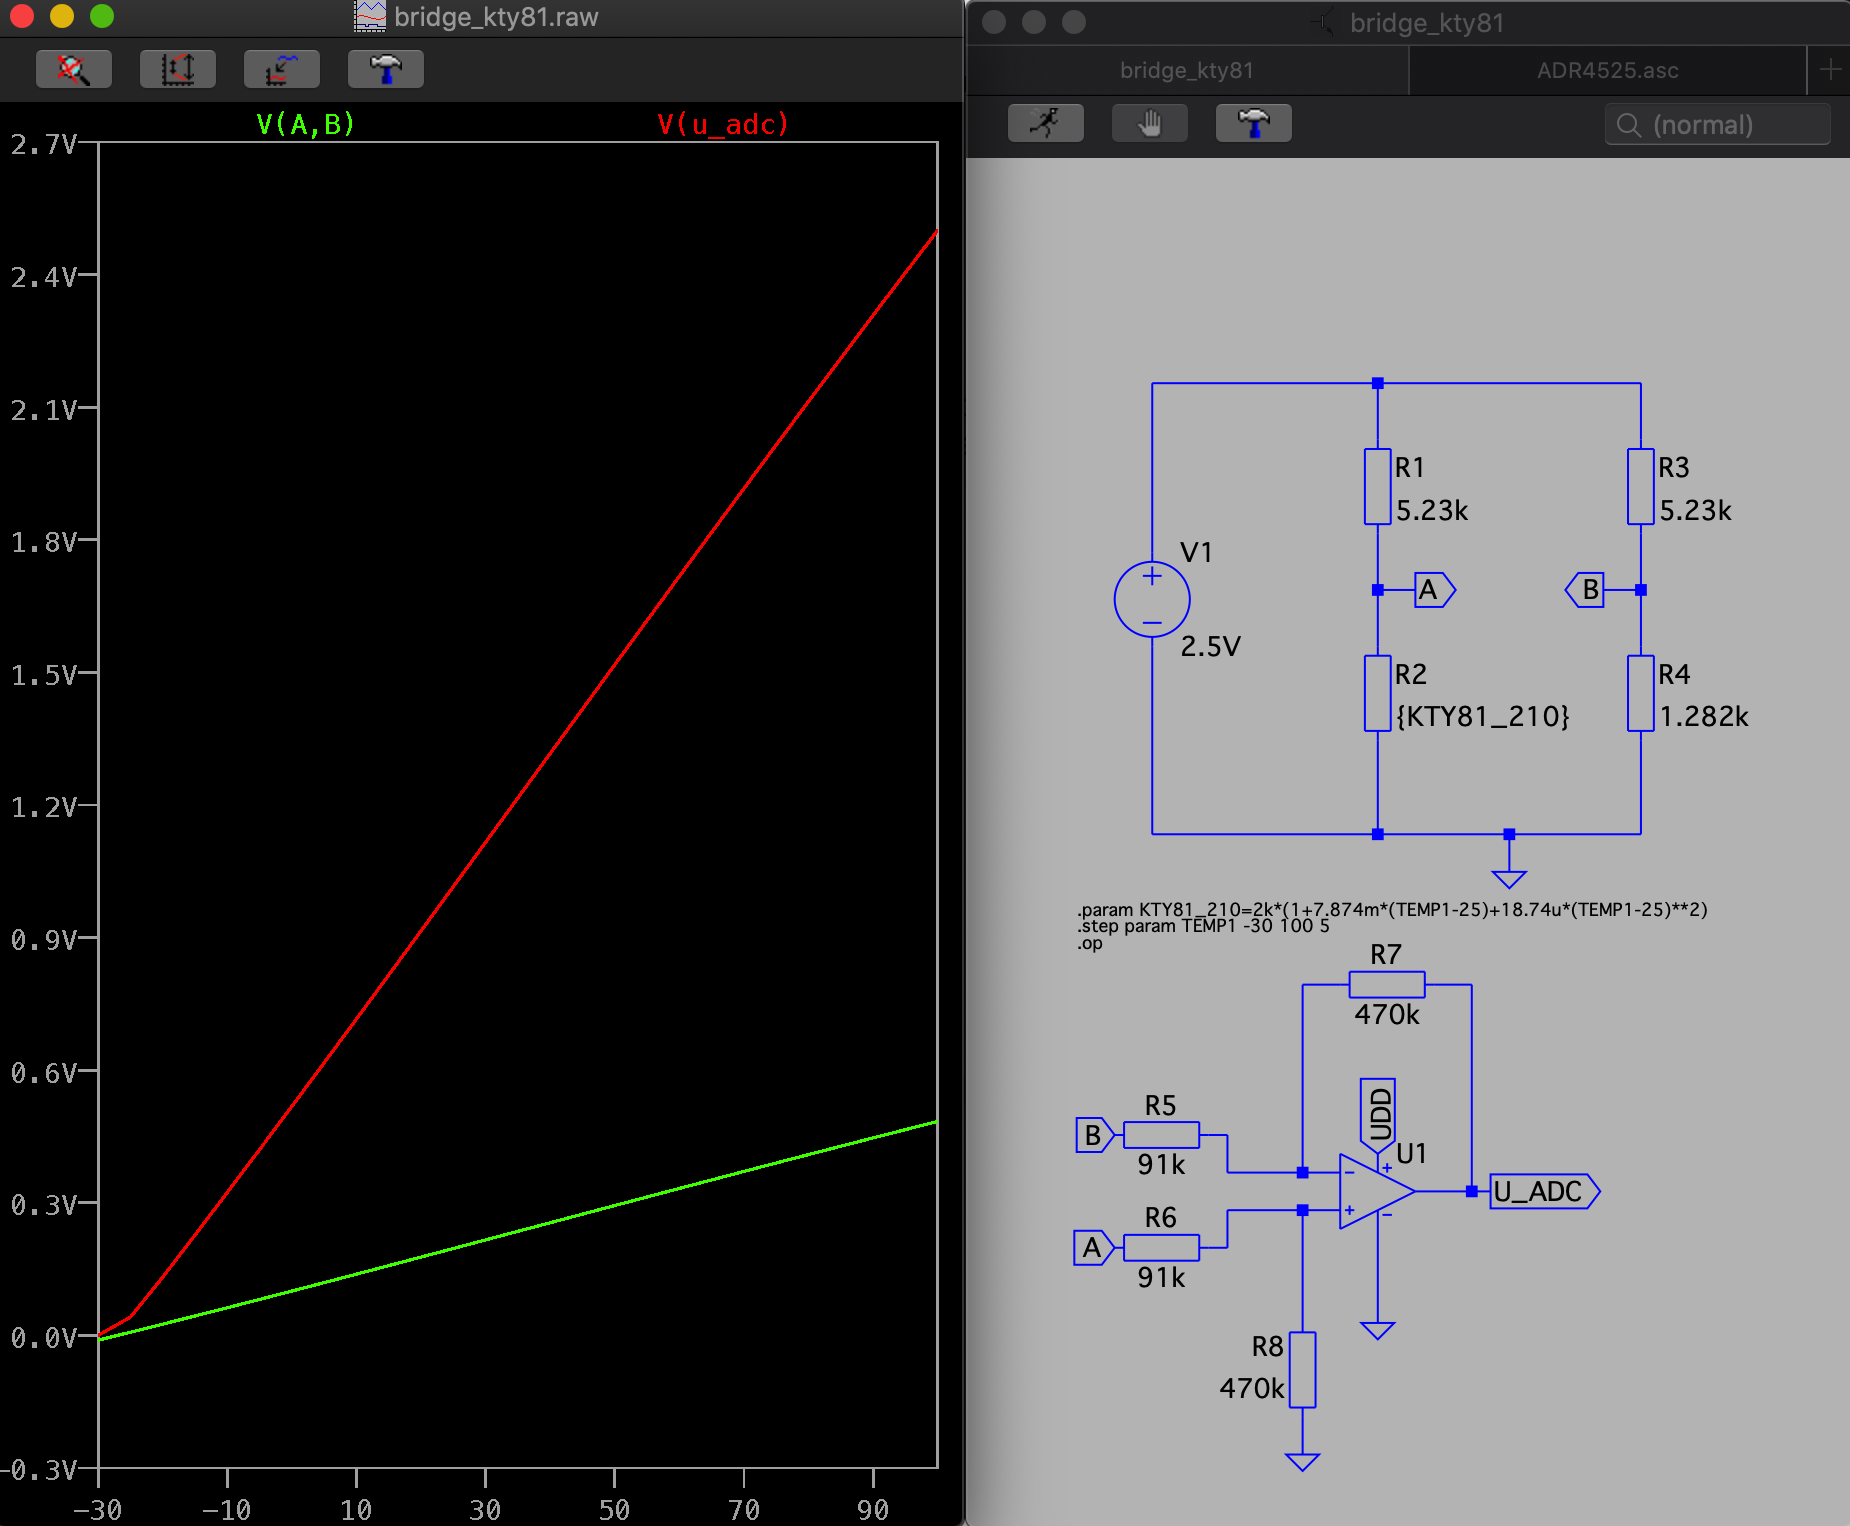
\includegraphics[width=0.5\linewidth]{pictures/diff_ampl_uadc_1.png}
            \end{figure}
        \end{minipage} 
    \end{tabular}

    \end{table}
     
    \end{tiny} \end{spacing}

\end{frame}

\begin{frame}[t]{Die Messbruecke - Alternative Anzeige am Digitalmultimeter} 
    
    \begin{spacing}{0.9} \begin{tiny}
      \begin{table}[h!]
      \begin{tabular}{p{10cm} }
        \hline
        \textbf{Potentailanpassung für das Multimeter} \\
        \hline \\
        \begin{minipage}{\textwidth}
           Alternativ kann die Spannung direkt an einem Digitalmultimeter angezeigt werden. \newline
           Das Digitalmultimeter soll jedoch idealerweise direkt die Temperatur ohne Umrechnungsfaktor anzeigen.
           \textbf{Wir haben einen nahezu idealen unsymmetrischen OPVs verwendet. Hier sehen wir, dass (wie auch bei einem realen TS912-5) die Kurve am Beginn des Messbereichs leicht abflacht. Daher limitieren wir den Messbreich bei -20C.}
           \begin{figure}
               \centering
               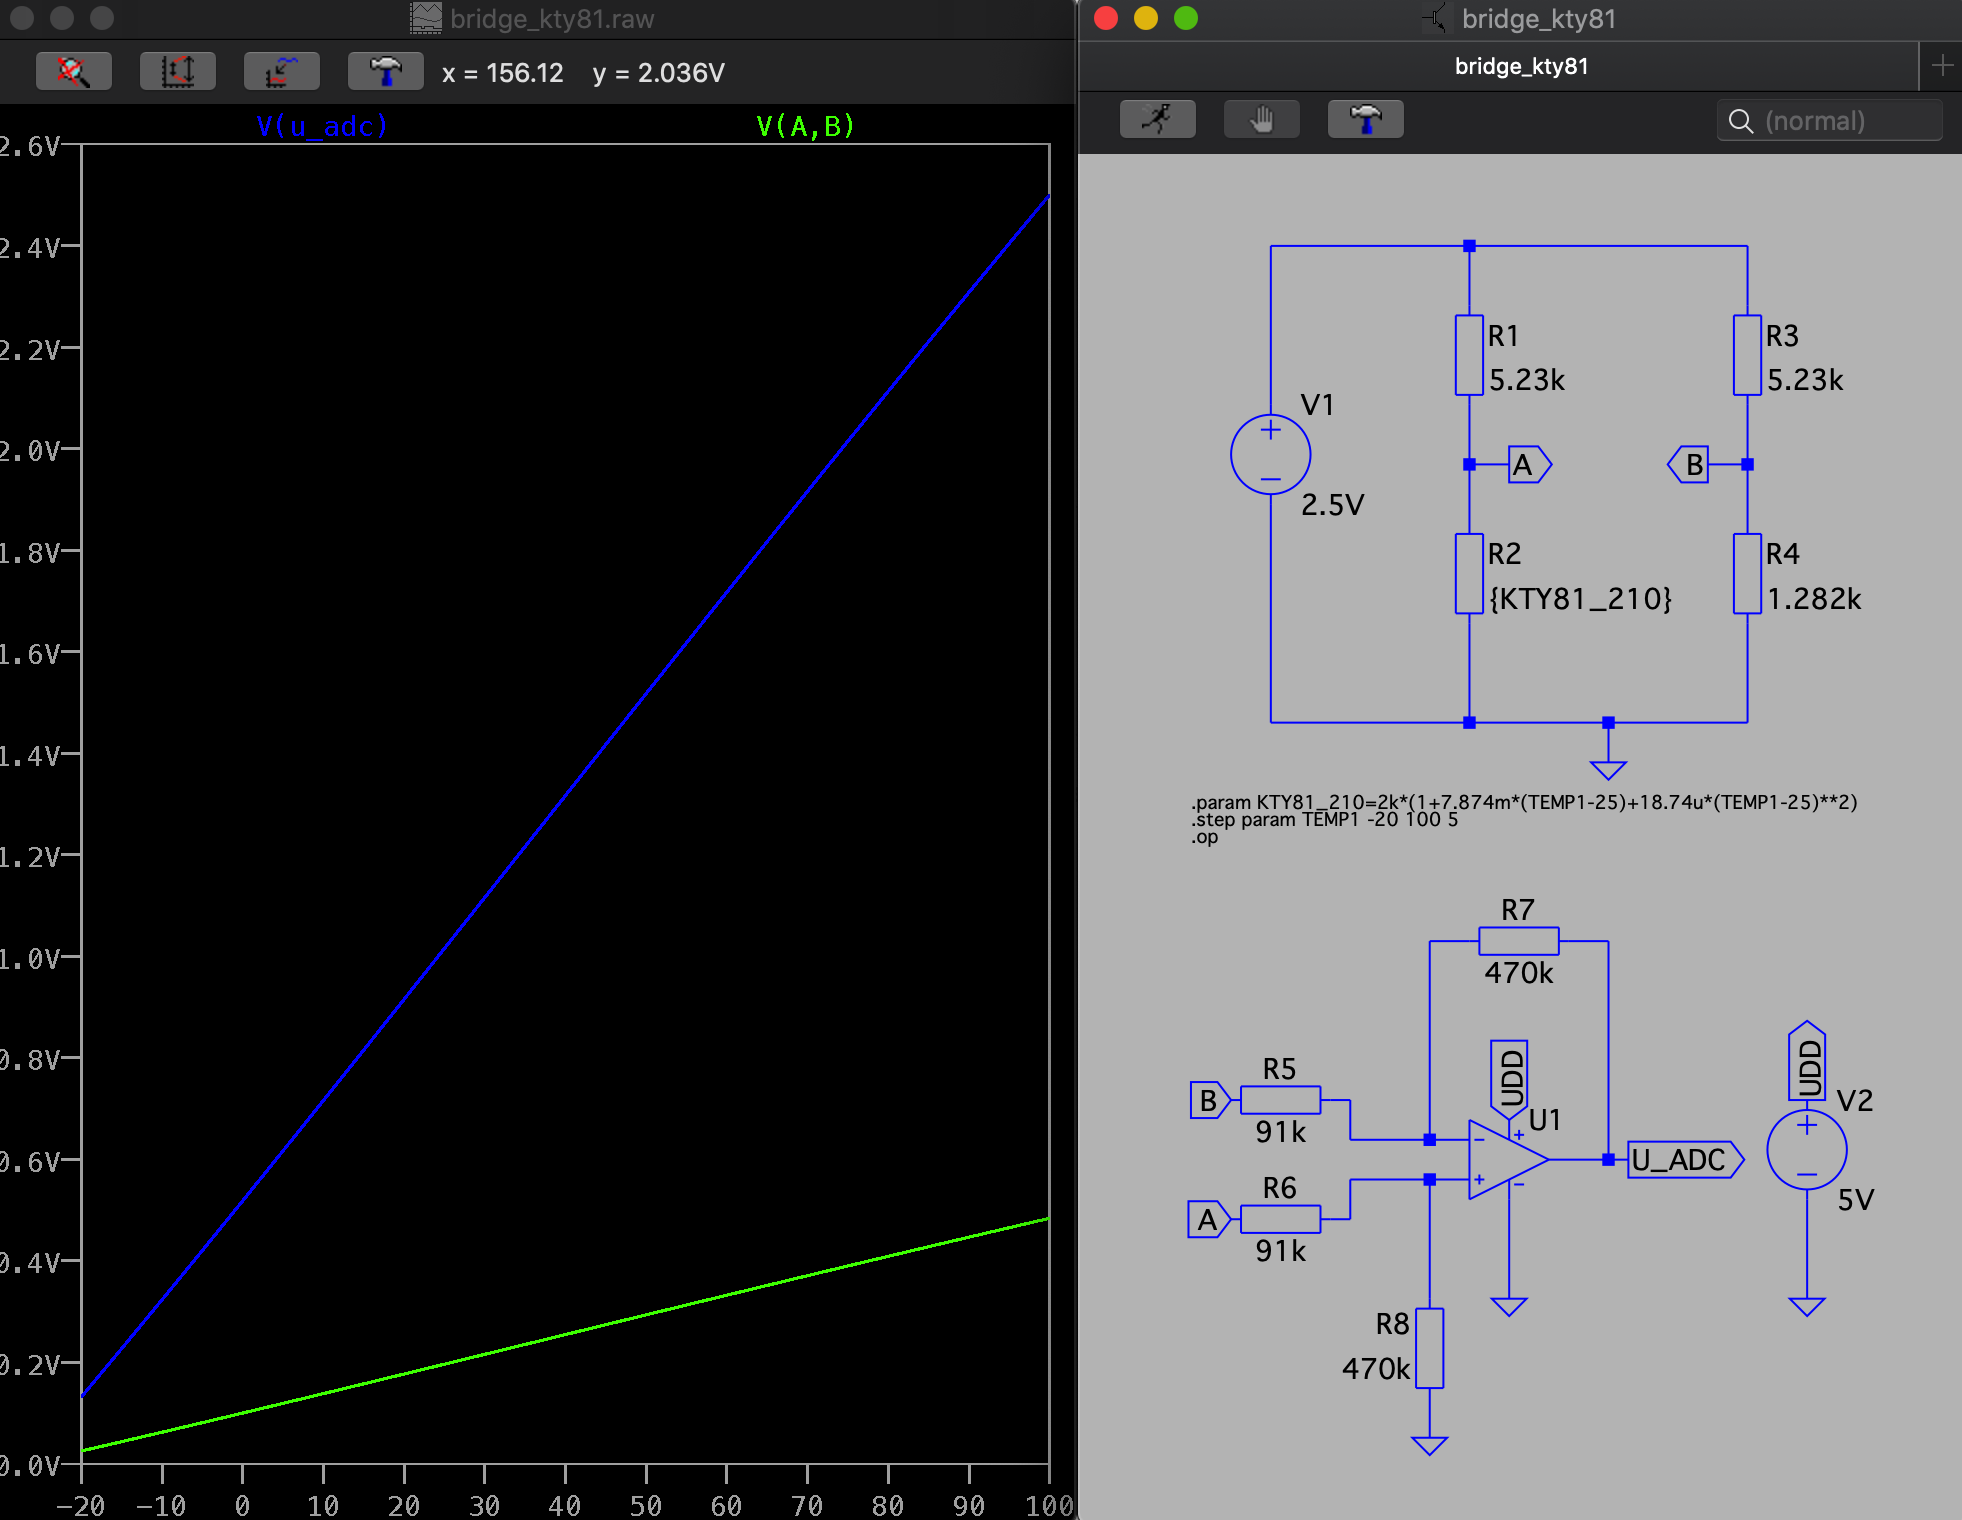
\includegraphics[width=0.4\linewidth]{pictures/digimul_ready.png}
           \end{figure}
           Um die Anpassung durchzuführen werden wir die folgenden Schritte abarbeiten um die Spannung der Temperatur anzugleichen:
           \begin{itemize}
               \item Spannungsteiler reduziert das Potential $U_{ADC}$
               \item Wir nutzen die temperaturkonstante Spannung $V_B$ mit einem weiteren Spannungsteiler um das Potential am negativen Messpunkt um 270mV zu senken
               \item \textbf{Für die Spannungsteiler müssen Potis zur initialen Einstellung verwendet werden, da es keine Widerstände in beliebigen Werten gibt. Jedenfalls nicht um unsere Spannungsteiler exakt zu dimensionieren.}
           \end{itemize}
        \end{minipage} 
    \end{tabular}

    \end{table}
     
    \end{tiny} \end{spacing}

\end{frame}

\begin{frame}[t]{Die Messbruecke - Alternative Anzeige am Digitalmultimeter} 
    
    \begin{spacing}{0.9} \begin{tiny}
      \begin{table}[h!]
      \begin{tabular}{p{10cm} }
        \hline
        \textbf{Schematic mit Modellierung von Potis} \\
        \hline \\
        \begin{minipage}{\textwidth}  
             \begin{itemize}
                 \item Spannungsteiler $U_{UAC} \frac{1,27}{2,5}=\thicksim 0,51$
                 \item $U_{B}=2,5(\frac{5,23k\Omega}{1,28k\Omega+5,23k\Omega})=0,492V=konstant$
                 \item Spannungsteiler $U_{B}=\frac{0,27}{0,492}=\thicksim 0,54$
                 \item $R_{Mess}$ sollte möglichst hochohmig dimensioniert werden.
             \end{itemize}
            \begin{figure}
                \centering
                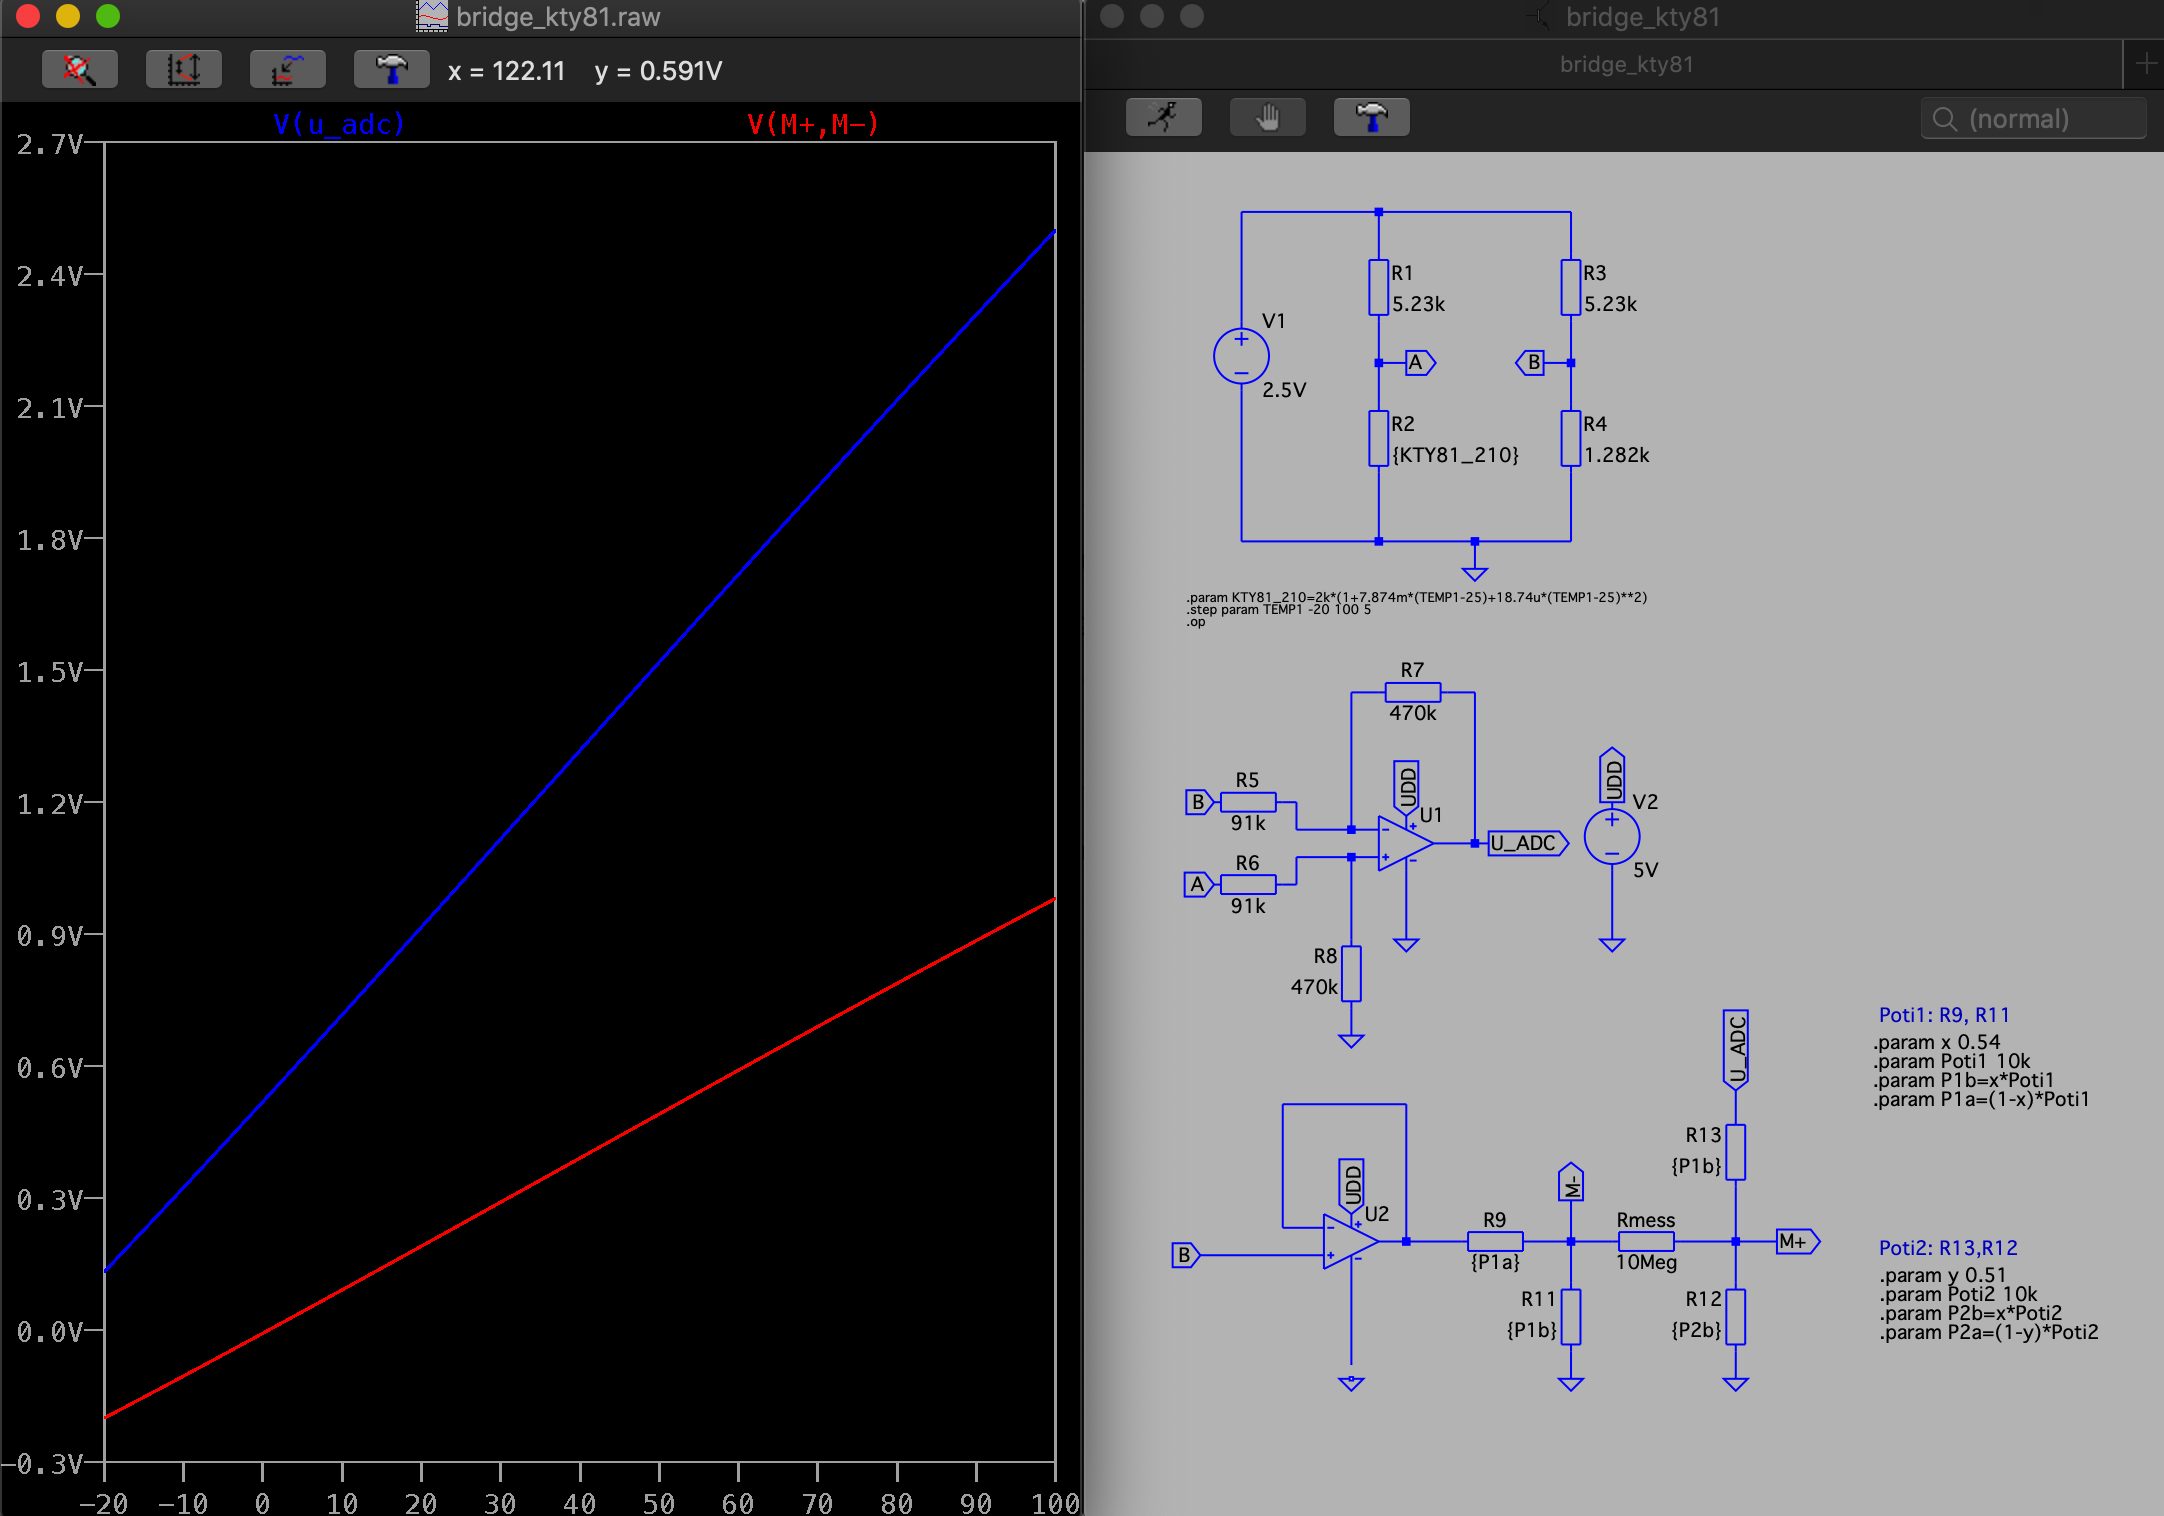
\includegraphics[width=0.7\linewidth]{pictures/digi_mul_anpassung.png}
            \end{figure}
        \end{minipage} 
    \end{tabular}

    \end{table}
     
    \end{tiny} \end{spacing}

\end{frame}

\begin{frame}[t]{Die Messbruecke - Die Referenzspannungsquelle} 
    
    \begin{spacing}{0.9} \begin{tiny}
      \begin{table}[h!]
      \begin{tabular}{p{10cm} }
        \hline
        \textbf{Verwendung eines realen Bauelementes} \\
        \hline \\
        \begin{minipage}{\textwidth}  
            Beim praktischen Schaltungsaufbau lässt sich die Referenzspannung mit einer Referenzdiode (z.B. direkt von analog devices ADR4525) 
            aus der Versorgungsspannung erzeugen. \textbf{Wir haben hier bisher eine ideale Spannungsquelle in der Simulation verwendet!}\newline
            \begin{figure}
                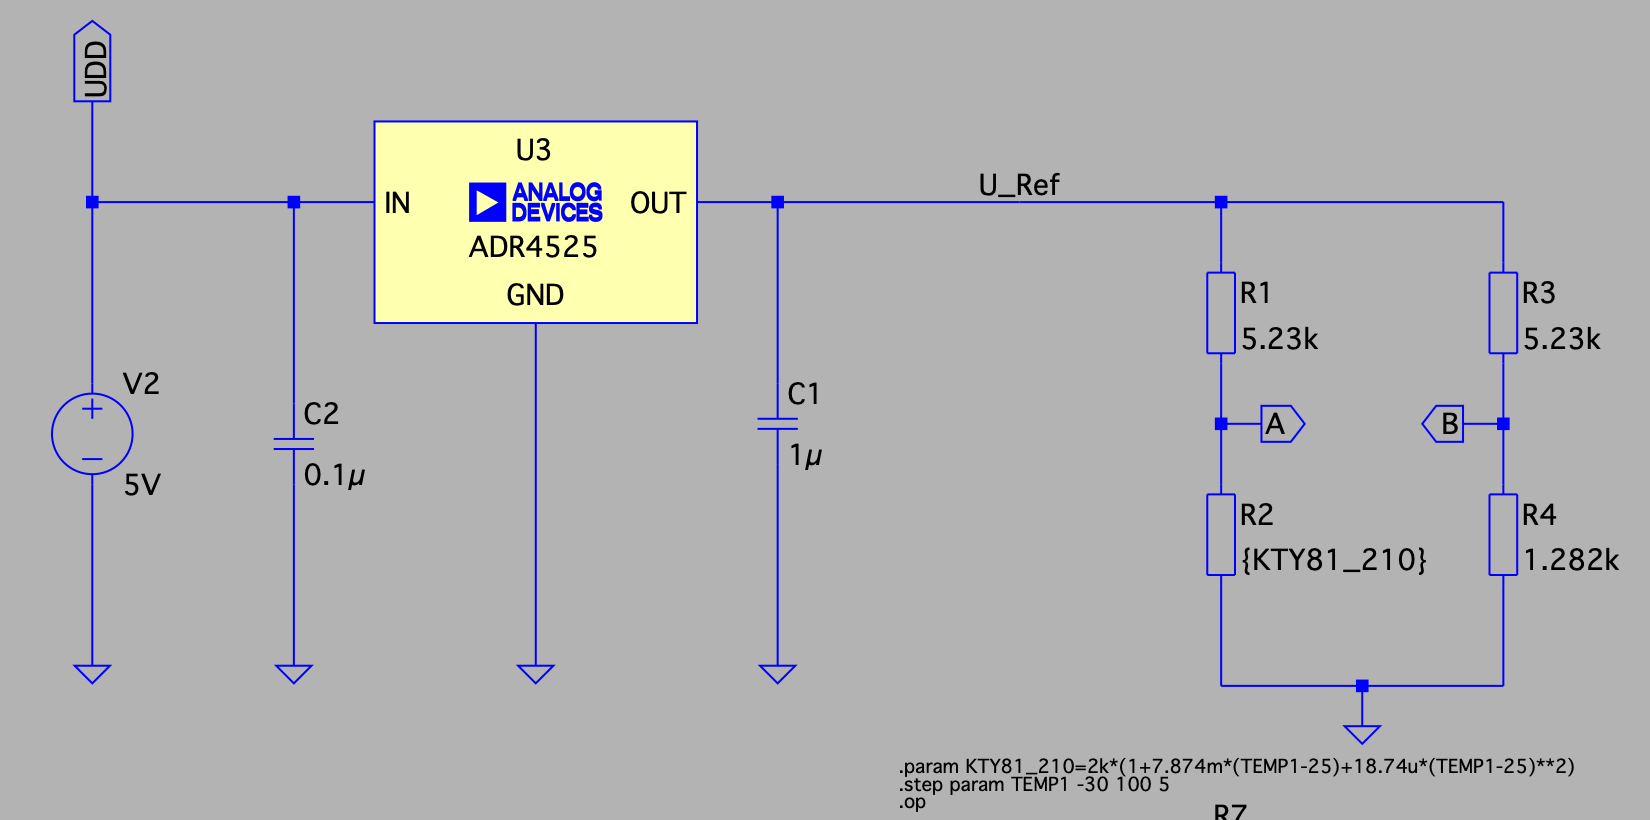
\includegraphics[width=0.8\linewidth]{pictures/uref.png}
            \end{figure}
            Im Vergleich zur Übersicht auf Folie 28, ist der LM285-2.5 nicht mehr in der Bauteilbibliothek verfügbar. 
            Daher haben wir hier zur realen Modellierung der Spannungsversorgung ein Bauteil von analog devices verwendet.
        \end{minipage} 
    \end{tabular}

    \end{table}
     
    \end{tiny} \end{spacing}

\end{frame}

\begin{frame}[t]{Die Messbruecke - Alles zusammen} 
    
    \begin{spacing}{0.9} \begin{tiny}
      \begin{table}[h!]
      \begin{tabular}{p{10cm} }
        \hline
        \textbf{-0,2 bis 1V bei Abgriff von M+ nach M-} \\
        \hline \\
        \begin{minipage}{\textwidth}  
            \begin{figure}
                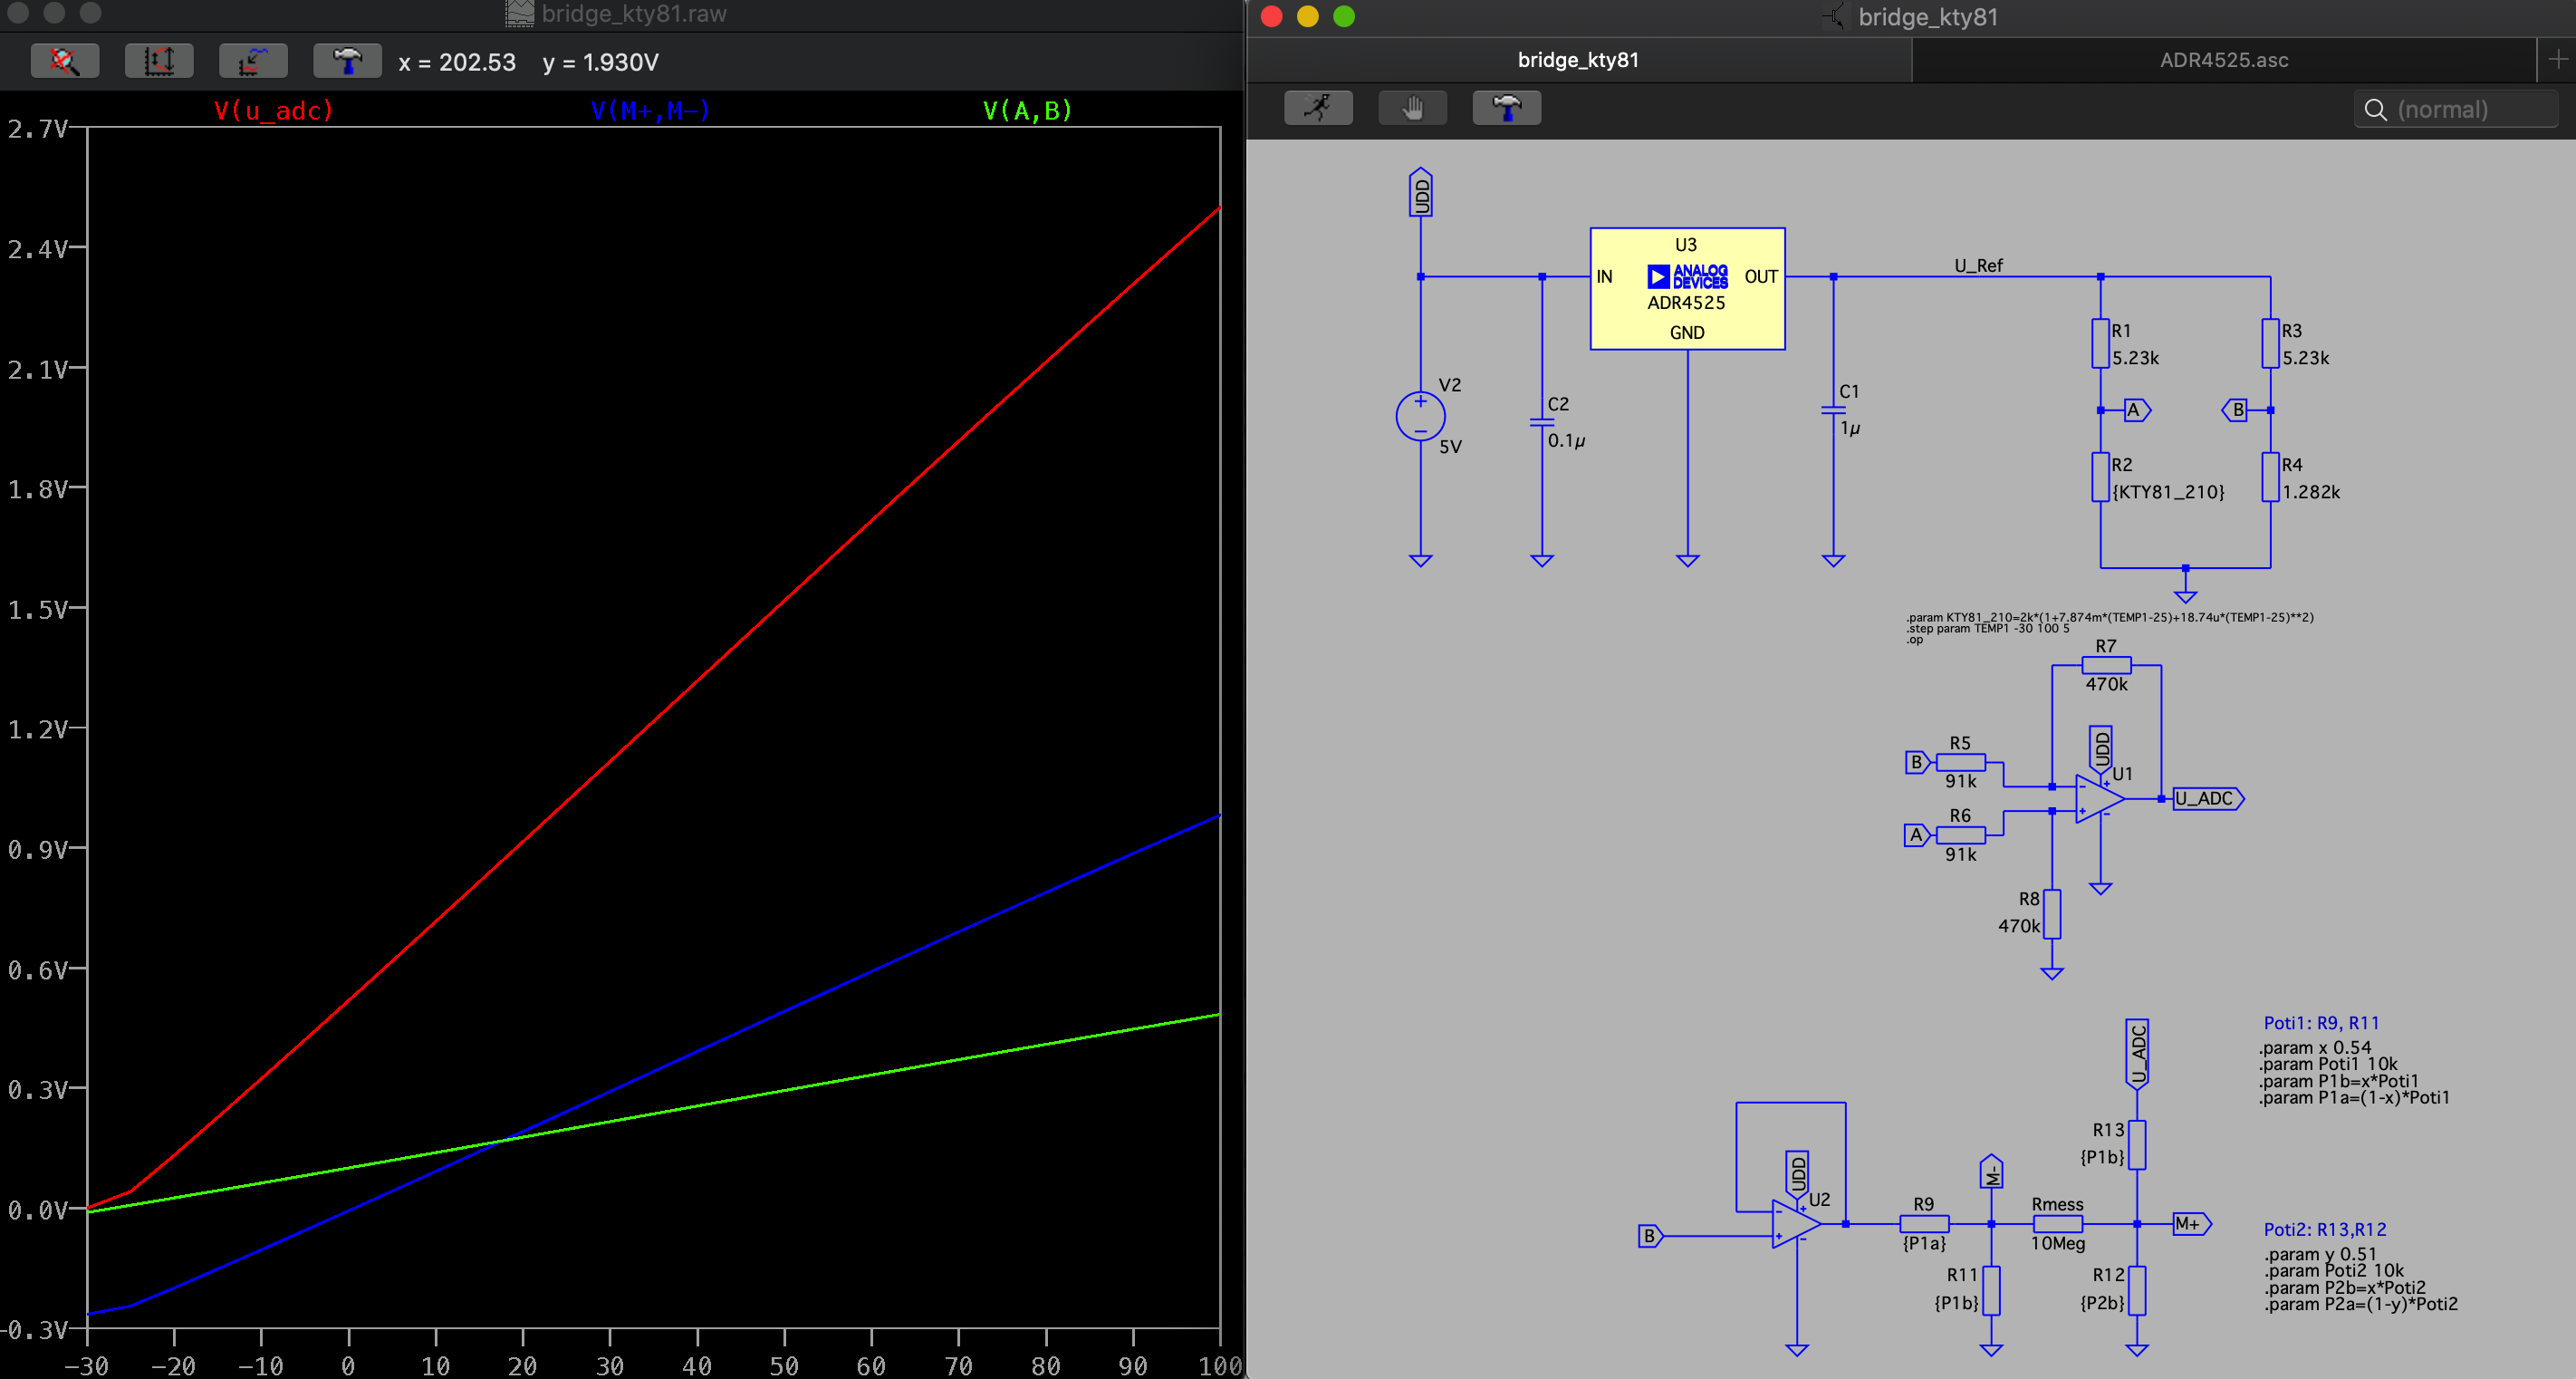
\includegraphics[width=\linewidth]{pictures/complete.png}
            \end{figure}
        \end{minipage} 
    \end{tabular}

    \end{table}
     
    \end{tiny} \end{spacing}

\end{frame}